\section{Hackenbush}

A Conway siempre le interesaron los juegos, era un jugador adicto al backgammon y de sus primeros aportes a la columna de Martin Gardner eran juegos que el hab\'ia creado, por ejemplo el juego Sprouts, creado por Conway en compa\~nia con el entonces estudiante de posgrado Mike Paterson, fue descrito en una carta que Conway le envi\'o a Gardner en 1967 y ese mismo a\~no Gardner la public\'o en su columna \cite{}.

Por eso, no es sorpresa, que al rededor del a\~no 1970, al descubrir el teorema de Sprague-Grundy, se obsesionara con los juegos. El teorema de Sprague-Grundy\cite{}, es un teorema que trata sobre los juegos imparciales, estos son aquellos juegos de informaci\'on perfecta, sin azar, tales que los movimientos posibles dependan solamente del tablero y no de qu\'e jugador est\'e jugando.

Vamos a explicar esta definici\'on parte por parte. Un juego de informaci\'on perfecta es un juego donde cada persona sabe cu\'ales movimientos pueden hacer los otros jugadores, en este sentido juegos como el p\'oker o el black-jack quedan descartados, puesto que los jugadores no saben qu\'e cartas tienen los otros. Un juego sin azar es un juego donde los movimientos no dependen del azar, no hay ning\'un dado que dicte los movimientos ni hay nig\'un generador de n\'umeros aleatorios que dicte el ganador, en este caso quedan descartados juegos como el parqu\'es, parch\'is o como la loter\'ia. La \'ultima condici\'on es la que le da el nombre de imparciales, esta es, si tenemos la posici\'on del tablero los movimientos posibles para los jugadores son los mismos, aqu\'i se descartan la mayor\'ia de otros juegos que se conocen, por ejemplo, el ajedrez tiene diferentes movimientos para los dos jugadores, uno juega con las fichas blancas y el otro con las fichas negras, o por ejemplo el triqui (tic-tac-toe), en este un jugador juega con las cruces (`X') y otro con los c\'irculos (`O'). F\'ijese en las figuras \ref{figure:game-chess} y \ref{figure:game-triqui}, en ambos tableros los posibles movimientos para las fichas negras y para las fichas blancas son diferentes, si le tocara jugar a un jugador ser\'ia este podr\'ia ganar, mientras que si le toca jugar al otro jugador este no tendr\'ia la posibilidad de ganar en ese movimiento.

\TwoFig{images/games-partisan-1.png} % image 1
         {Tablero de ajedrez donde el jugador con las fichas negras puede ganar en un movimiento, pero el jugador con las blancas no. \textit{(Fuente: lichess.com)}} % caption 1
         {figure:game-chess} % label 1
         {images/games-partisan-2.png} % image 2
         {Tablero de triqui donde el jugador con las `X' puede ganar en un movimiento, pero el jugador con las `O' no. \textit{(Google)}} % caption 2
         {figure:game-triqui} % label 2

Un ejemplo de juego al que s\'i se le puede aplicar el teorema de Sprague-Grundy, es decir un juego imparcial, es el comunmente juego 21. En el juego se van turnando entre dos personas, el primer jugador dice el n\'umero `1' y el siguiente jugador tiene que aumentar el n\'umero en `1', `2' o `3'. Pierde el jugador que diga `21' o un n\'umero mayor que `21'. Un ejemplo de c\'omo un juego de `21' puede pasar es:

\begin{center}
    \begin{tabular}{|c|M{3cm}|}
        \hline
        Jugador & \text{N\'umero} \\
        \hline\hline
        1 & 1 \\
        \hline
        2 & 4 \\
        \hline
        1 & 7 \\
        \hline
        2 & 10 \\
        \hline
        1 & 11 \\
        \hline
        2 & 13 \\
        \hline
        1 & 16 \\
        \hline
        2 & 17 \\
        \hline
        1 & 20 \\
        \hline
        2 & 21 \\
        \hline
    \end{tabular}
\end{center}

Ac\'a el jugador 1 gan\'o porque el jugador 2 dijo 21. F\'ijese que en este juego las opciones para los dos jugadores son las mismas, el `tablero' de este juego consistir\'ia en el n\'umero que se ha dicho inmediatamente en el turno anterior.

El teorema de Sprague-Grundy le asigna un valor a todos los juegos de este tipo con el que se puede calcular qu\'e jugador va a ganar (jugando de la mejor manera), si el primero o el segundo. Adem\'as de todo, el teorema da una forma en la que se pueden calcular valores de juegos que consisten en la combinaci\'on de otros juegos m\'as simples, por ejemplo, si quisieramos jugar dos juegos imparciales al mismo tiempo pero en cada turno solo podr\'iamos hacer un movimiento en uno de los dos juegos, el teorema de Sprague-Grundy nos dir\'ia como calcular qui\'en ganar\'ia con base a los valores de cada uno de los juegos imparciales.

Conway quer\'ia generalizar este teorema pero para juegos m\'as generales, los llamados juegos partisanos. Los juegos partisanos son tambi\'en juegos sin azar y de informaci\'on perfecta, pero en este caso no tenemos la condici\'on extra de imparcialidad, entonces entran juegos como el ajedrez, el triqui o el go.

En la \'epoca de 1970 sucedieron var\'ias cosas que ayudaron al estudio de estos juegos. Primero, Jon Diamond, el campe\'on brit\'anico de Go durante 11 a\~nos \cite{}(https://www.britgo.org/people/diamondj), entr\'o a estudiar matem\'aticas en Cambridge. \'El fund\'o la \textit{Cambdridge Go Society} y con eso incentiv\'o el juego dentro de Cambridge.
Conway se interes\'o por el Go principalmente porque los juegos de Go tienen la propiedad de que casi al final de la partida, el tablero se separa en ciertas zonas, casi como si se estuvieran jugando varios juegos simultaneamente, cada jugador eligiendo en cada turno en qu\'e parte jugar.

La otra cosa que ayud\'o al desarrollo de la teor\'ia fue el inter\'es de Richard Guy y Edwin Berlekamp


\begin{figure}[h]
    \centering
    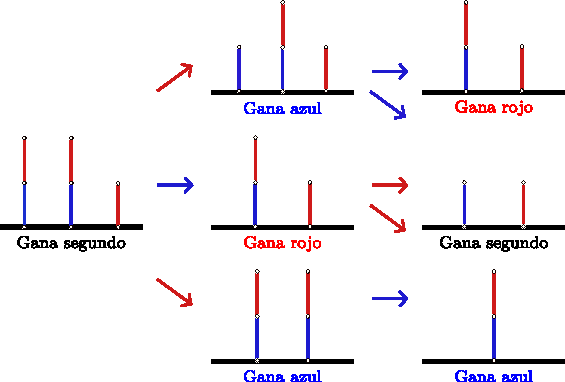
\includegraphics[width=.7\textwidth]{images/hackenbush-half_proof.pdf}
\end{figure}